% !TEX root = ../main.tex
\paragraph{Drift Chambers (DC)}
    \begin{wrapfigure}{r}{0.50\textwidth}
        \centering\frame{
        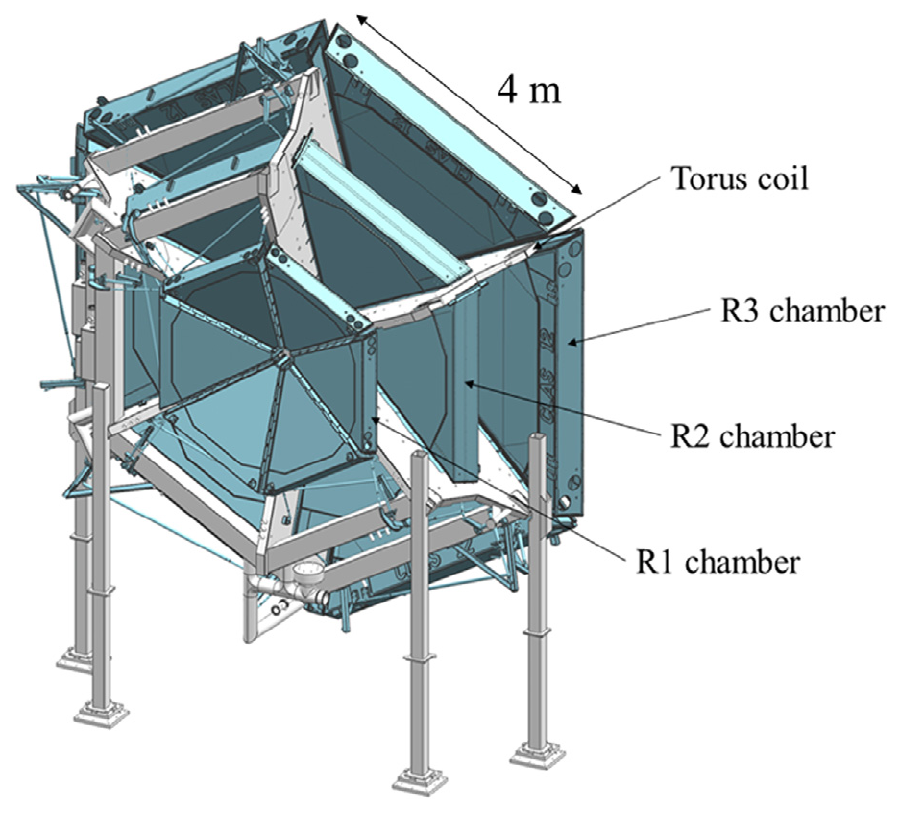
\includegraphics[width=\linewidth]{212dc.png}}
        \caption[DC]{Drift Chambers render.
        Each of the DC regions are denoted as R1, R2, and R3 in the figure.}
        \label{fig::dc}
    \end{wrapfigure}

    The six coils of the torus magnet act as support for the forward tracking system, which consists of three independent drift chambers in each of the six sectors of the torus magnet.
    Each of the six DC sectors has a total of 36 layers with 112 sense wires each, arranged in three regions of twelve layers each.
    In each of the six torus sectors, the drift chambers are arranged identically.
    The arrangement of the DC around the torus coil can be seen in Figure \ref{fig::dc}

    As can be seen on the figure, the first region is located at the entrance to the torus magnetic field region.
    Then, the second is inside the magnet, where the magnetic field is close to its maximum.
    The third is located in a low magnetic field space, just downstream of the torus magnet.
    This arrangement provides independent and redundant tracking in each of the six torus sectors.

    Each of the three regions consists of six ``superlayers'', each of which contains two layers.
    One layer has wires strung at a stereo angle of $+6\degree$ while the second one of $-6\degree$, both with respect to the sector midplane.
    This stereo view enables excellent resolution in the polar angle ($\Delta\theta < 2 ~\text{mrad}$), and good resolution in the azimuthal scattering angle ($\Delta\phi < 2 ~\text{mrad}$).

    The DC can detect ionising particles with momenta above $200 ~\text{MeV}/\text{c}$, with a $\Delta p/p$ lesser than $0.5\%$.
    This offers a track momentum resolution of $3$ to $5\%$ \cite{mestayer2020}.
